%!TEX root = ./main.tex

\section{Future work}\label{section:future_work}

There are three areas of future work I plan to explore in the next year before defending my thesis.

\paragraph{Benchmarking} Chapter~\ref{section:global_methods} includes a number of preliminary results suggesting that gradient-based inference methods perform well on a range of challenging robotics problems, including problems with poorly-conditioned gradients (flat regions and discontinuities). However, it is not yet clear what underlying factors contribute to this performance. In the next year, I will perform a series of experiments to both ablate different aspects of gradient-based inference methods and apply them to problems with different challenging features (including discontinuities, stiff gradients, subgradients, and inaccurate gradients). The goal will be to develop practical guidance for when practicioners can expect gradient-based inference methods to perform well.

Specifically, this research will proceed in four stages:
\begin{enumerate}
    \item Define a suite of state-of-the-art optimization and inference algorithms, including gradient-free and gradient-based methods, including ablations of particular methods.
    \item Define a suite of benchmark problems with the ability to scale aspects like problem dimension, number and extent of discontinuities, number of distinct modes, etc..
    \item Conduct benchmarking experiments to compare the performance of different algorithms on different problems.
    \item Using results from benchmarking, infer practical checks that can be used to determine whether a problem is suitable for gradient-based inference methods, and compile these checks into a software package that can be used by practitioners.
\end{enumerate}

\paragraph{Probabilistic programming} In my work in Chapter~\ref{section:global_methods}, I combine automatic differentiation with gradient-based inference on programs with a specific structure $J(S(x, y))$. The decision to factor out all uncertainty into the inputs $y$ makes easier to apply approximate inference algorithms, but it enforces a fixed topology on the underlying probabilistic graphical model (requiring graphical models with the structure shown on the left in Fig.~\ref{ch7:fig:graphical_models}). This restricted set of structures restricts the expressiveness of the probabilistic model, in particular making it difficult to model interactions between exogenous parameters (as in the example structure shown on the right in Fig.~\ref{ch7:fig:graphical_models}). In the next year, I will explore how to remove this restriction through the use of a fully-features probabilistic programming language such as Gen~\cite{Cusumano-Towner:2019:GGP:3314221.3314642}. Using such a language, it is possible to define programs that make random choices without factoring out the uncertainty (instead, special syntax is used to annotate random choices as they occur in the code).

\begin{figure}[b]
    \centering
    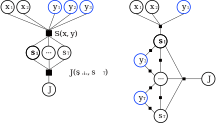
\includegraphics[width=0.8\linewidth]{images/ch7/graphs.png}
    \caption{Left: a factored graphical model in the form supported by the inference methods presented in Chapter~\ref{section:global_methods}, where all random choices (blue circles) are factored out into the exogenous inputs $y$. Right: a graphical model with a more complex structure, where random choices are not factored out and can depend on intermediate states.}
    \label{ch7:fig:graphical_models}
\end{figure}

In particular, this research will explore two distinct questions:
\begin{enumerate}
    \item Can we use probabilistic programming to perform causal analysis of autonomous systems, in particular answering root-cause failure analysis problems? E.g. if a robot fails to complete a task in a particular way, can we use probabilistic programming to infer the most likely cause or causes of the failure?
    \item Can we use probabilistic programming to define inference problems that search over the space of possible program structures? E.g. to search over the space of possible robot limb morphologies, or to search over symbolically-defined control policies? This will involve drawing on recently-developed methods for involutive and reversible-jump MCMC, which have been applied to inference problems with hierarchical models~\cite{cusumano-townerAutomatingInvolutiveMCMC2020}.
\end{enumerate}

% Explain gap between existing approach (reparameterization trick/factor out all randomness into inputs to deterministic function) and probabilistic programming.

% Explain advantages that probprog may have for a design process.

% Formulate specific research goal.

\paragraph{Lessons learned for gradient-free solution methods}

A large part of this thesis is motivated by the ability to introspect program structure (e.g. through automatic differentiation) to improve the performance of design and verification algorithms. Unfortunately, there will always be problems where it is not feasible to perform this introspection; for example, if a simulator relies on proprietary code that is only available in binary form, or if there is simply not enough engineering effort available to port an existing simulator to an AD-compatible library. To handle these cases, in the next year I will explore how to apply the lessons learned from gradient-based design and verification to accelerate gradient-free solution methods, including through the use of gradient estimation and proxy modeling.

The main output of this line of research will be a gradient-free MCMC inference algorithm that uses a combination of proxy modeling and gradient estimation to accelerate convergence to the target distribution. This algorithm will be evaluated on a range of challenging problems, including problems with stiff gradients, discontinuities, and flat regions.
